\section{Summary of the Proposal}

Sparse matrices are extensively used in scientific computing, however there is no automatic differentiation package in Julia yet to handle sparse matrix operations yet. This project will utilize the reversible embedded domain-specific language NiLang.jl to differentiate sparse matrix operations by re-writing the sparse functions in Julia base in a reversible style. I will port the generated backward rules to ChainRules.jl as an extension, where ChainRules.jl is the most popular Julia package providing backward rules for automatic differentiation packages. 

\section{Background}

\par Matrices having only a small percentage of nonzero elements are said to be sparse. Sparse matrices have been applied in many areas: e.g., linear programming, network theory, structural analyses and so on. Recently, the automatic differentiation (AD) on sparse matrices has become a popular topic in the scientific computing field. Modern AD packages depoly a broad range of computational techniques to improve applicability, run time, and memory management. Most of the well-known AD packages in the market, such as Tensorflow, Pytorch and Flux implement reverse mode AD and checkpointing techniques at the tensor level to meet the need in deep learning.  

\par However, sometimes scientists and engineers have to define backwards rules manually for specific scientific problems, such as Hamiltonian engineering, phase transition problem and so on. Instead of defining backward rules manually, one can also use a general purposed AD (GP-AD) framework like Tapenade, Zygote and NiLang\cite{liu2020differentiate}. NiLang, a reversible domain-specific language, shows its great potential in generating backward rules for sparse matrices. In this project, we will implement AD for sparse matrix operations by rewriting programs in Julia base by NiLang. Furthermore, backward rules generated by NiLang will be ported to ChainRules.jl as an extension. 

\section{Goal and Objectives}
\label{sec:goals}
The main target of this project is providing AD for sparse matrices by NiLang. It could be broken into three concrete goals as following:
\begin{itemize}
    \item Implement sparse matrix operations in Julia writen by NiLang.
    \item Generate chain rules and export them into ChainRules.jl.
    \item Release an open source Julia package on AD for sparse matrices. Test converage should be above 80\% and a quick start tutorial for the package should be presented.
\end{itemize} 

\section{Methods}
In this section, we will give a detailed introduction to design and techniques in this project. We will talk about the data structure of sparse arrays in Julia first. Then we will propose how to construct AD for sparse matrices from low level operations to high level operations. Finally we consider about exporting chain rules generated by reversible functions into ChainRules.jl. 
\subsection{SparseCSC}
Julia has support for sparse vectors and sparse matrices in the \href{https://docs.julialang.org/en/v1/stdlib/SparseArrays/}{SparseArrays stdlib module}. As mentioned before, sparse arrays are arrays that contain enough zeros. To take advantage of this special property, sparse arrays are stored in a special data structure, known as  \href{https://en.wikipedia.org/wiki/Sparse_matrix#Compressed_sparse_column_.28CSC_or_CCS.29}{Compressed Sparse Column (CSC) format}, which leads to great savings in space and execution time compared to dense arrays.

\begin{figure}
    \begin{center}
        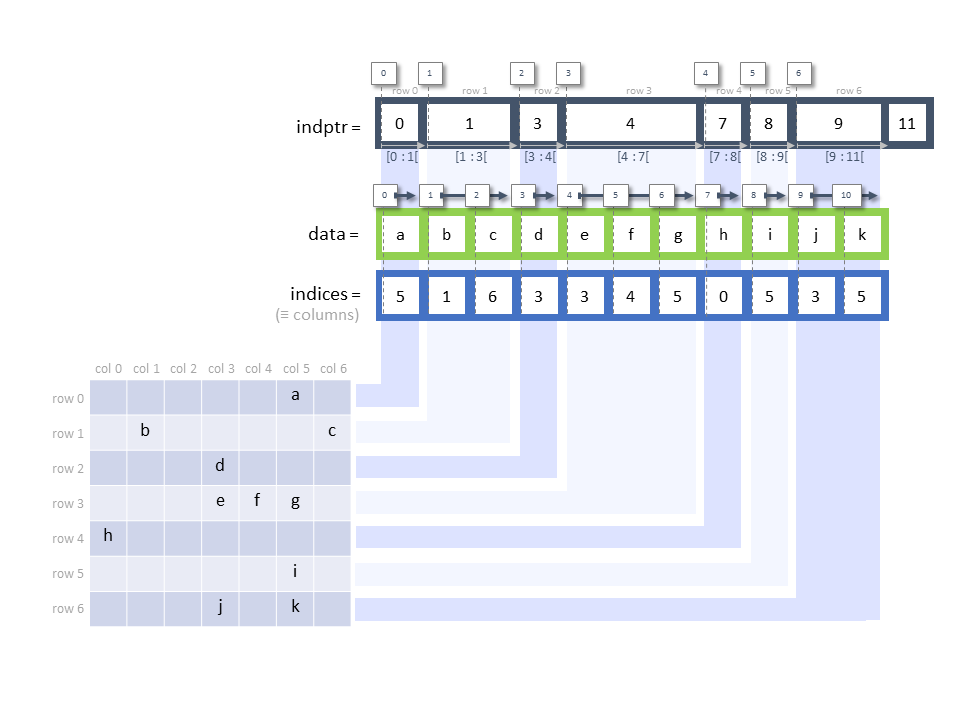
\includegraphics[width = .8\linewidth]{pic/SPCSC.png}
        \caption{SparseCSR Format Illustration}
    \end{center}
\end{figure}

The internal representation of SparseMatrixCSC in Julia is as follows:
\begin{lstlisting}[language=Julia]
    struct SparseMatrixCSC{Tv,Ti<:Integer} <: AbstractSparseMatrixCSC{Tv,Ti}
    m::Int                  # Number of rows
    n::Int                  # Number of columns
    colptr::Vector{Ti}      # Column j is in colptr[j]:(colptr[j+1]-1)
    rowval::Vector{Ti}      # Row indices of stored values
    nzval::Vector{Tv}       # Stored values, typically nonzeros
    end
    \end{lstlisting}

In this project, we will fully exploit the SparseMatrixCSC format to improve the performance of sparse matrix operations, e.g. matrix multiplication. Elements in columns of sparse matrix would be accessed more often whereas elements in rows of sparse would be accessed less to avoid slow operations. I mentioned and analyzed this performance gap in  \href{https://jieli-matrix.github.io/sparsecsc/}{my blog }. 

\subsection{Low Level Operations}

Low level operations are reffered as basic matrix operations in matrix computation, e.g. BLAS. SparseArrays module in Julia provides a large amount of low level operations in \href{https://github.com/JuliaLang/julia/blob/master/stdlib/SparseArrays/src/linalg.jl}{linalg.jl}. It could be summarized into several categories as following:

\begin{lstlisting}[language=Julia]
    function mul!(C::StridedVecOrMat, A::AbstractSparseMatrixCSC, B::DenseInputVecOrMat, α::Number, β::Number)
    function dot(A::AbstractSparseMatrixCSC{T1,S1},B::AbstractSparseMatrixCSC{T2,S2}) where {T1,T2,S1,S2}
    function kron(C::SparseMatrixCSC,A::AbstractSparseMatrixCSC,B::AbstractSparseMatrixCSC)
    function norm(A::AbstractSparseMatrixCSC, p::Real=2)
\end{lstlisting}
Low level operations above would be implemented by NiLang in the development plan. It should be addressed that low level operations are the basis in this project since it will not only provide interface to users directly but also provide support for high level operation.


\subsection{High Level Operations}
High level operations are reffered as operations exploiting the structure of a matrix, e.g. matrix decomposition. Matrix decomposition plays an important role in matrix computation, one of the most famous matrix decomposition is singular value decomposition (SVD). 
\par However, SVD causes great computation when the scale of matrix is tremendous. Instead of implementing classical SVD for sparse matrices by NiLang, we would implement low rank SVD and linear Principal Component Analysis (PCA) for them. Such probabilistic algorithms would project the original sparse matrix $\mathbf{A}$ into a smaller matrix $\mathbf{B}$ and perform SVD on $\mathbf{B}$ so as to save computation. 
\par In order to make familar with the project, I implemented the low rank SVD algorithm in \href{https://github.com/jieli-matrix/Lowranksvd.jl/tree/dev}{Lowranksvd.jl}. It served as an important reference for the implementation by NiLang.  

\subsection{Export Chain Rules into ChainRules.jl}
We would export chain rules into ChainRules.jl when we accomplished the task of rewriting sparse matrix operations by NiLang. The delicate design of NiLang makes it easy to generate the back propogation process and gradient by calling $\sim$ \textit{reversible\_function}.
\par We could obtain the gradient of norm function by NiLang as following\footnote[1]{\url{https://github.com/GiggleLiu/NiLang.jl/blob/master/examples/port_chainrules.jl}}:
\begin{lstlisting}[language=Julia]
    using NiLang, NiLang.AD, Zygote, ChainRules
    using BenchmarkTools
    # Julia native implementation of `norm2` function.
    function norm2(x::AbstractArray{T}) where T
        out = zero(T)
        for i=1:length(x)
            @inbounds out += x[i]^2
        end
        return out
    end
    # Then we have the reversible implementation
    @i function r_norm2(out::T, x::AbstractArray{T}) where T
        for i=1:length(x)
            @inbounds out += x[i]^2
        end
    end
    x = randn(1000);
    @benchmark (~r_norm2)(GVar($(norm2(x)), 1.0), $(GVar(x))) seconds=1

\end{lstlisting}

We could generate chain rules in a reverse mode by binding the reversible function to ChainRules.rrule and export it into ChainRules.jl as following
\begin{lstlisting}[language=Julia]
norm2_faster(x) = norm2(x)
function ChainRules.rrule(::typeof(norm2_faster), x::AbstractArray{T}) where T
    out = norm2_faster(x)
    function pullback(ȳ)
        ChainRules.NoTangent(), grad((~r_norm2)(GVar(out, ȳ), GVar(x))[2])
    end
    out, pullback
end

original_grad = norm2'(x)
@assert norm2_faster'(x) ≈ original_grad
\end{lstlisting}

\section{Schedule and Timeline}

This project will be shipped by four (mostly) sequential stages:
\begin{enumerate}[(1)]
    \item Implement low level operations by NiLang.
    \item Implement high level operations by NiLang.
    \item Export chain rules into ChainRules.jl. 
    \item Release the project. Add more documentation and tutorials.
\end{enumerate}

For the purpose of OSPP phase evaluation, I’ll list the expected timeline of this project in the form of Gantt chart \cite{gantt1910work}
\begin{enumerate}[(1)]
    \item 1st Jul - 31st Jul \quad Implement low level operations by NiLang. Carefully test by CI and export chain rules into ChainRules.jl.
    \item 1st Aug - 30th Aug   \quad Implement high level operations by NiLang. Carefully test and export chain rules into ChainRules.jl.
    \item 1st Sep - 20th Sep \quad Release the project. Add more documentation and tutorials.
    \item 21st Sep - 30th Sep \quad Leave the time as flexible week. 
\end{enumerate}
\vspace{0.5cm}

\noindent\resizebox{\textwidth}{!}{
\begin{tikzpicture}[x=.5cm, y=1cm] 
\centering
        \begin{ganttchart}[%Specs
            y unit title=0.4cm,
            y unit chart=0.5cm,
            canvas/.style={fill=none, draw=black, line width=.75pt},
            vgrid,
            title label anchor/.style={below=-1.6ex},
            title left shift=.05,
            title right shift=-.05,
            title height=1,
            title/.style={fill=none},
            title label font=\bfseries,
            bar/.style={fill=barblue},
            incomplete/.style={fill=white},
            progress label text={},
            bar height=0.7,
            group right shift=0,
            group top shift=.6,
            group height=.3,
            group peaks height=.2]{1}{36}

            %labels
            \gantttitle{2021}{36}\\
            \gantttitle{Jul}{12}
            \gantttitle{Aug}{12}
            \gantttitle{Sep}{12}
            \\

            % Parameter Selection
            \ganttgroup{Stage 1}{2}{12}\\ %elem0
            %\ganttbar[progress=0]{sub-objective}{2}{18}\\
            \ganttmilestone{Low-Level Ops}{6}\\\\

            % Testing equipment
            \ganttgroup{Stage 2}{13}{25}\\ %elem0
            %\ganttbar[progress=0]{Bar}{2}{18}\\
            \ganttmilestone{CI and ChainRules}{18}\\\\

            % Testing
            \ganttgroup{Stage 3}{26}{32}\\ 
            %\ganttbar[progress=0]{Bar}{19}{35}\\
            %\ganttbar[progress=0]{Bar}{19}{35}\\
            \ganttmilestone{High-Level Ops}{29}\\
            %\ganttmilestone{Milestone}{35}\\

            % Algorithm Development
            \ganttgroup{Stage 4}{33}{35}\\
            \ganttmilestone{Merge}{34}\\ 
            %\ganttbar[progress=0]{Bar}{28}{35} \\

            %relations 
            %\ganttlink{elem2}{elem6}
            %\ganttlink{elem5}{elem6}
            %\ganttlink{elem9}{elem11}

        \end{ganttchart}
    \label{fig:Gantt2014}
\end{tikzpicture}}  

\vspace{0.5cm}  


OSPP 2021 has two evaluation phases, this is a reference criterion that I have in mind; whether it is adopted depends on mentors’ own judgement:

\begin{itemize}
    \item Phase 1 \quad Student and mentor should submit the phase 1 evaluation before 15th Augst. As long as the implementation of low level operations have been accomplished and passed CI building, it should be considered sufficient to pass.
    \item Phase 2 \quad Student and mentor should submit the final phase evaluation before 30th September
    . It should be considered a pass once 1. all sparse matrix operations in the development plan have been implemented with test converage above 80\% 2. there are specific documentation, tutorials.
\end{itemize}